\documentclass{article}
\usepackage[utf8]{inputenc}
\usepackage{graphicx}
\usepackage{hyperref}
%\usepackage[a4paper,width=150mm,top=1in,bottom=1in]{geometry}
%\usepackage[a4paper,margin=1in]{geometry}
\usepackage{indentfirst}

\usepackage{amsmath}
\pagenumbering{arabic}
\usepackage{subcaption}
\usepackage[numbered]{mcode}    %using mcode.sty to convert .m file code to latex format
\usepackage{listings}
\usepackage{adjustbox}
\usepackage{minted}
\usepackage{mathtools}
\usepackage{multicol}
\graphicspath{{./images/}}

\lstset{
  basicstyle=\ttfamily,
  columns=fullflexible,
  frame=single,
  breaklines=true,
  postbreak=\mbox{\textcolor{red}{$\hookrightarrow$}\space},
}

\begin{document}

\begin{titlepage}
    % --------------------------------------------------------------------
    % Formatting title layout
    % --------------------------------------------------------------------
    \newcommand{\HRule}[1]{\rule{\linewidth}{#1}} 	% Horizontal rule
    \makeatletter							% Title
    \def\printtitle{%						
        {\centering \@title\par}}
    \makeatother									
    
    \makeatletter							% Author
    \def\printauthor{%					
        {\centering \large \@author}}				
    \makeatother							

    % --------------------------------------------------------------------
    % Title text
    % --------------------------------------------------------------------
    \title{	\normalsize \textsc{} 	% Subtitle
    		 	\\[2.0cm]								% 2cm spacing
    			\HRule{0.5pt} \\						% Upper rule
    			\LARGE \textbf{\uppercase{Lab 1\\ Audio Filtering on Time Domain Signals in MATLAB}}	% Title
    			\HRule{2pt} \\ [0.5cm]		% Lower rule + 0.5cm spacing
    			\normalsize Digital Signal Processing II\\
    			ECE 161B | WINTER 2020\\
    			\today			% Todays date
    		}
    
    \author{
    		Roy Kim\\	
    		A13804992\\
    		Electrical and Computer Engineering\\	
    		UC San Diego\\
    }
    
    % ------------------------------------------------------------------------------
    % Title display (Maketitle)
    % ------------------------------------------------------------------------------
    \thispagestyle{empty}		% Remove page numbering on this page
    
    \printtitle					% Print the title data as defined above
      	\vfill
    \printauthor				% Print the author data as defined above
    \newpage

\end{titlepage}

% ------------------------------------------------------------------------------
% Table of contents
% ------------------------------------------------------------------------------
\hspace{0pt}
\vfill
\tableofcontents
\vfill
\hspace{0pt}
\newpage
% ------------------------------------------------------------------------------
% Content
% ------------------------------------------------------------------------------
\section{Introduction}
    In this lab we will construct the \textit{Twinkle Twinkle Little Star} song using sinuoidal tones that we will create. We will realize an IIR-Filter from the given difference equation and identify the filter type. Then we will pass our input signals, which will be the songs, through the filter. We will be implementing this process, first using MATLAB, then using C. The results will be compared by listening to the generated WAV file and by observation of their respective spectrograms. Another means for a comparison value that will be used in this lab to assess the result, is by normalizing the two songs and obtaining the relative error.

%    \begin{figure}[h!]
%        \centering
%        \includegraphics[scale=1.7]{universe}
%        \caption{The Universe}
%        \label{fig:universe}
%    \end{figure}

\section{Objectives}
    \begin{enumerate}
      \item Compose a song
      \item Perform filter operations on the time domain signal
    \end{enumerate}

\section{Results}
    \subsection{Task 1.} Generate a time domain signal of each note in the melody. Given $F_s=8000$ and $L=0.5$
        \begin{center}
            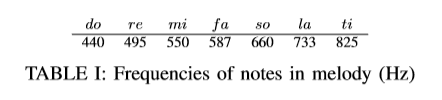
\includegraphics[scale=0.8]{table1.PNG}
        \end{center}
        \begin{align*}
            x=sin(2\times pi\times f\times t);
        \end{align*}
        
        \indent We are given a sampling rate $F_s=8000$ samples per second and the duration of each note to be $L=0.5$ seconds. So each note will have $F_s\times L=4000$ samples per note. So we can take 4000 sample of a sinusoid at the corresponding note frequency, sampling at $F_s$, to generate a 0.5 second tone. Doing this for each note in the melody, we get seven individual tones.
        \pagebreak
        
    \subsection{Task 2.} Use MATLAB's \textit{spectrogram()} function on the signal. Describe how the spectrogram  validates your implementation.\\
        
        \begin{center}
            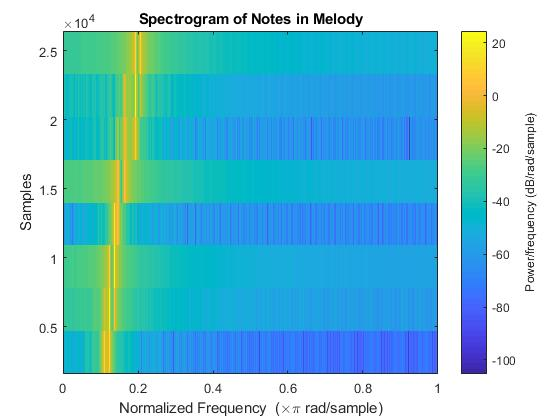
\includegraphics[width=\textwidth]{task2.jpg}
        \end{center}
        MATLAB's \textit{spectrogram($signal$)} function generates a time-frequency representation of the $signal$. The spectrogram shows the time the frequency is active. By concatenating the notes in the given melody and observing its corresponding spectrogram, we can verify what frequencies are being played with respect to time. Re-plotting the figure above with respect to time in seconds and frequency in kilo hertz as seen below.
        \begin{center}
            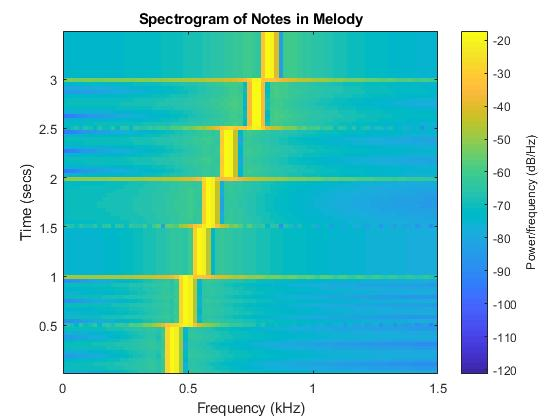
\includegraphics[width=\textwidth]{task2b.jpg}
        \end{center}
        We can observe that frequencies between 400Hz to 900Hz are being played within a time-span of 3.5 seconds. This aligns with the seven melody notes in an increasing frequency order; each with a duration of 0.5 seconds, with a total of 3.5 seconds.
        
    \subsection{Task 3.} Generate the melody and chorus of \textit{Twinkle Twinkly Little Stars}. Then form the complete song by combining the melody and chorus. Write the result to a WAV file.\\
        \vspace{5mm}\\
        Given the notes in the melody and chorus to be the following,
        \begin{center}
            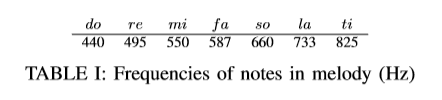
\includegraphics[scale=0.8]{table1.PNG}
            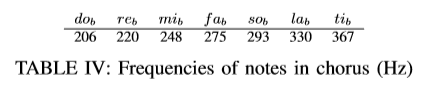
\includegraphics[scale=0.8]{table4.PNG}
        \end{center}
        \begin{center}
            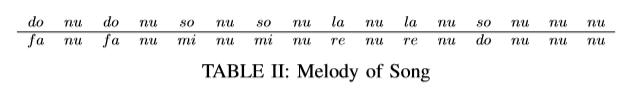
\includegraphics[width=\textwidth]{table2.PNG}
            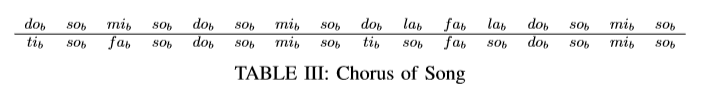
\includegraphics[width=\textwidth]{table3.PNG}
        \end{center}
        We are able to create a tone for each note by generating sinusoids of each individual note into a vector. Using the notes, we compose the songs of the melody and chorus by constructing a matrix. Each row of the matrix corresponds to the musical note being played in the order given in table II and each column of the matrix corresponds to the sample of the sinusoid at that particular frequency. Using this method, we construct a 32x4000 matrix corresponding to the 32 notes in the song and the 4000 sample for each note to have a duration of 0.5 seconds sampled at 8000 samples per second. We can then convert this matrix into a single row by taking its transpose and reshaping it into a row vector. The result is a single row vector that has each note concatenated at the end of each previous note in the order given by its song. This row vector has $32*4000=128000$ columns, so we have composed the 32-note song in a 1x128000 row vector. Doing this for the melody and the chorus of the song, we can then sum the two to compose a complete song of \textit{Twinkle Twinkle Little Stars} by playing the melody with the chorus.
        \begin{align*}
            x=0.6x_{melody}+0.4x_{chorus}
        \end{align*}
        
        
    \subsection{Task 4.} Generate a spectrogram of the complete song ($x$)\\
        \vspace{5mm}
        \begin{center}
            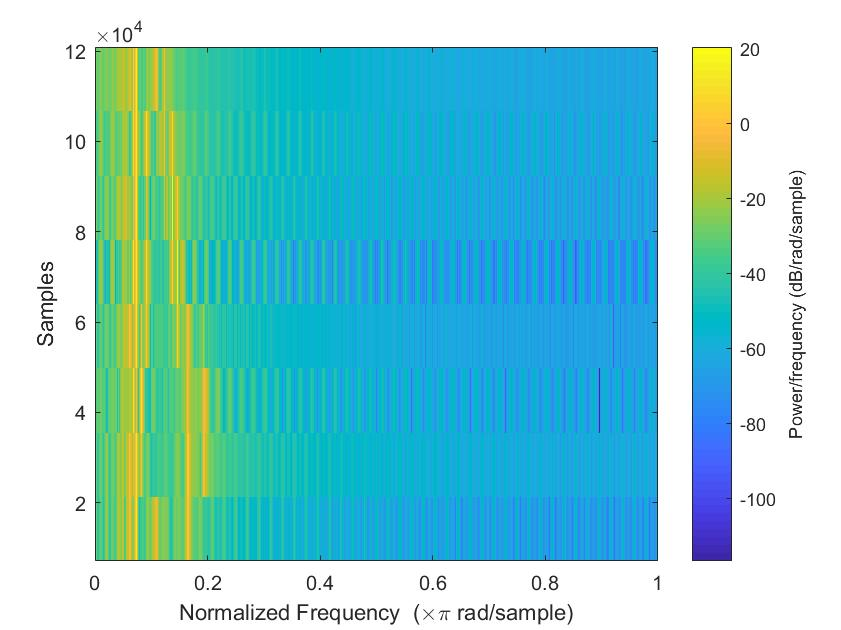
\includegraphics[scale=0.25]{task4.jpg}
        \end{center}
        \begin{center}
            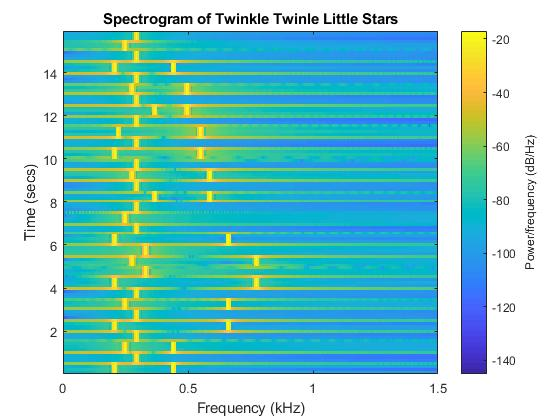
\includegraphics[width=\textwidth]{task4b.jpg}
        \end{center}
        The spectrogram verifies that the song is playing both the melody and chorus simultaneously. From the spectrogram, we can observed two tones being playing at the same time instance. And this is due to the overlap in time of the melody and chorus. We can also know that the melody frequencies are higher than the chorus frequencies. And it can be observed that the higher frequency components, which belong to the melody, are brighter colored (have higher power). This is due to the higher amplitude we assigned to the melody components when creating the complete song.
        
    \subsection{Task 5.} Create the given IIR filter. Then pass the song through the filter.\\
        \vspace{5mm}\\
        Create an IIR filter $h$ which can be described as,
        \begin{center}
            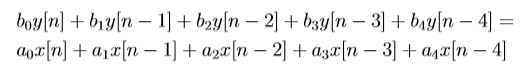
\includegraphics[width=\textwidth]{filter.PNG}
        \end{center}
        \pagebreak
        Realization of the IIR-filter above,\\
        \indent Pad zeros before the signal to account for causality. Then using the difference equation, we can find the values for $y[n]$ element-by-element-wise iterating in a loop. Due to causality, we know that the signal is 0 when $n<0$.
        \begin{align*}
            \hline
            \vspace{2mm}\\
            y[0]&=a_0x[0]\\
            y[1]&=a_0[1]+a_1x[0]-b_1y[0]\\
            y[2]&=a_0x[2]+a_1x[1]+a_2x[2]-b_1y[1]-b_2y[0]\\
            ...\\
            y[4]&=a_0x[4]+a_1x[3]+a_2x[2]+a_3x[1]+a_4x[0]-b_1y[3]-b_2y[2]-b_3y[1]-b_4y[0]\\
            \vspace{2mm}\\
            \hline
            \vspace{2mm}\\
            y[n]&=a_0x[n]+a_1x[n-1]+a_2x[n-2]+a_3x[n-3]+a_4x[n-4]\\
            &-b_1y[n-1]-b_2y[n-2]-b_3y[n-3]-b_4y[n-4]\\
            \vspace{2mm}\\
            \hline
        \end{align*}
        IIR Filter funtion in MATLAB,
        \lstinputlisting[frame=single]{code-files/IIR_filter_h.m}
        \vspace{5mm}\\
        Spectrogram of the filtered signal,
        \begin{center}
            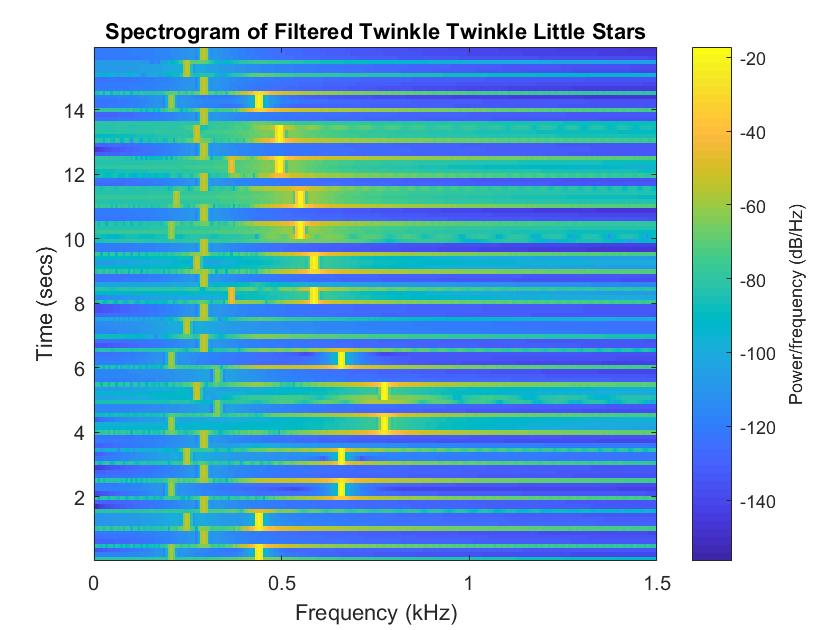
\includegraphics[width=\textwidth]{task5spectro.jpg}
        \end{center}
        From the spectrogram of the filtered signal, we can see that the lower frequency components, corresponding to the chorus, has been attenuated--decreased in power. This can be visually seen by the decrease in the yellow color from the low frequency signal components.
        
    \subsection{Task 6.} Generate a magnitude response plot of the IIR filter.\\
        \begin{center}
            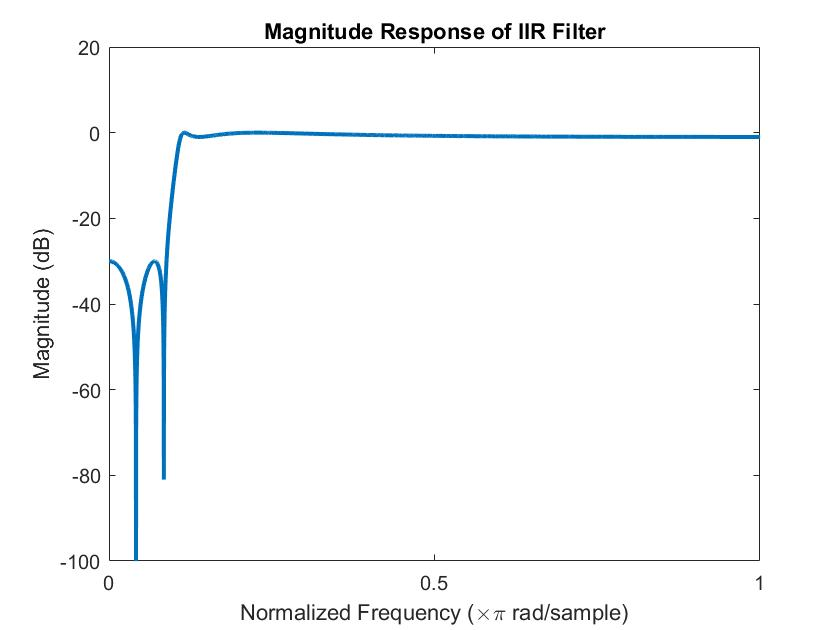
\includegraphics[width=\textwidth]{task6.jpg}
        \end{center}
        The magnitude response plot of the implemented IIR filter shows a filter design that filters out the low frequency components of the signal--Components near 0 and 2$\pi$. So the implemented IIR filter is a high pass filter. From the filtered audio sound, we can hear the melody clearly and the chorus filtered out. The magnitude response tells us that the melody has been unaltered (gain of 0dB) as the signal is passed through the filter, while the chorus has been attenuated (negative gain). This is expected since the chorus is played at a lower frequency than the melody frequency. When listening to the sound played by the filtered signal, it sounds as if it was played on the piano using only the right hand--the higher frequency keys.\\
        \vspace{5mm}\\
        Confirming with the pole-zero plot of this IIR filter. We can expect to see at least four zeros corresponding to the zeros near 0 and 2$\pi$ as seen in the magnitude response plot.
        \begin{center}
            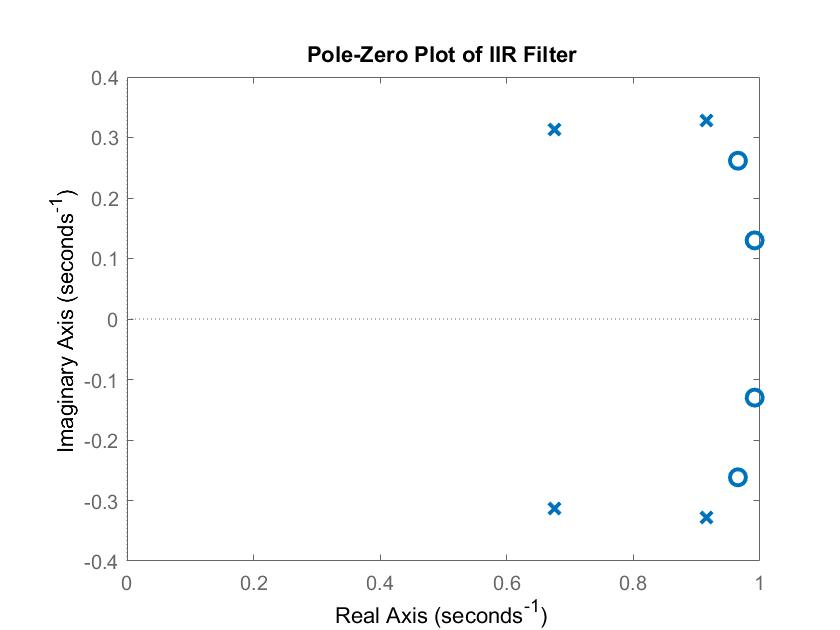
\includegraphics[width=\textwidth]{task6vera.jpg}
        \end{center}
        The pole-zero plot confirms our expectation of the IIR filter. The four zeros are near 0 and 2$\pi$, attenuating low frequencies, while the poles are at a slightly higher frequency to bring the magnitude response back to unity, gain of 0dB. The pole-zero plot also shows us that the zeros are at the low frequency side; where the right side (0 and 2$\pi$) maps to the low frequency and the left side ($\pi$) maps to the high frequency.
    
    \subsection{Task 7.} Generate the song \textit{Twinkle Twinkle Little Star} in a C program. Write the result to a WAV file. Read the WAV file into in MATLAB and compare with the MATLAB result using relative error as the distance measure.\\
        \vspace{5mm}\\
        Spectrogram of C-program's non-filtered output WAV file is shown below,
        \begin{center}
            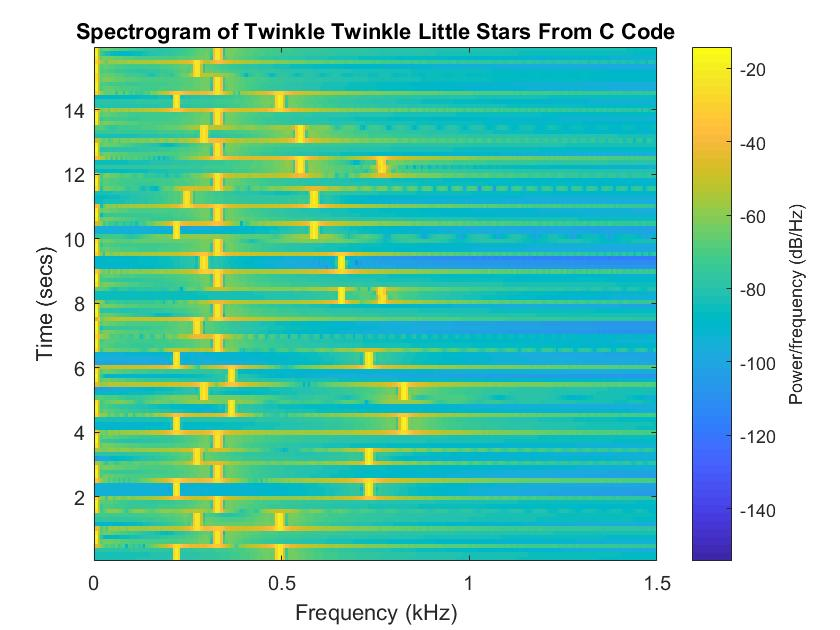
\includegraphics[width=\textwidth]{task7.jpg}
        \end{center}
        Below is a side-by-side comparison between MATLAB implementation (right figure) and C implementation (left figure),
        \begin{center}
            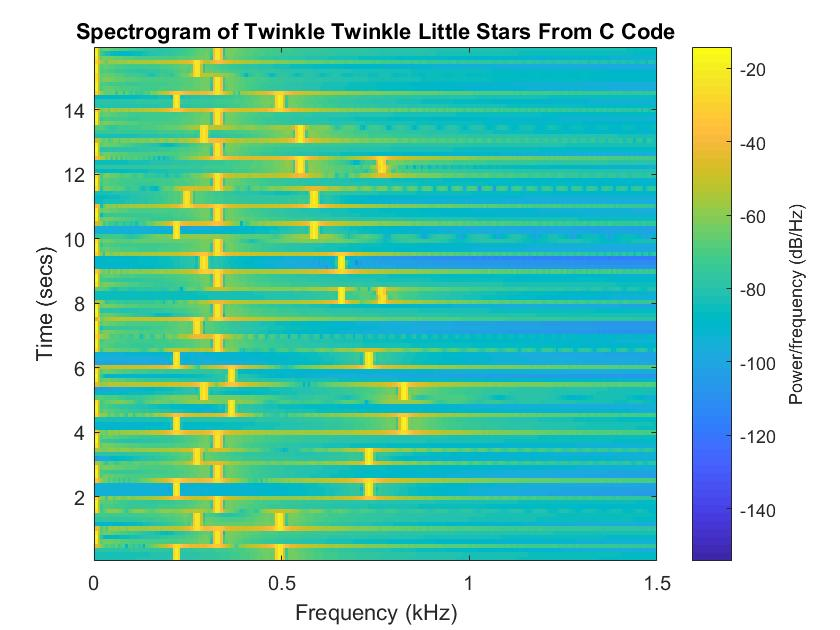
\includegraphics[scale=0.2]{task7.jpg}
            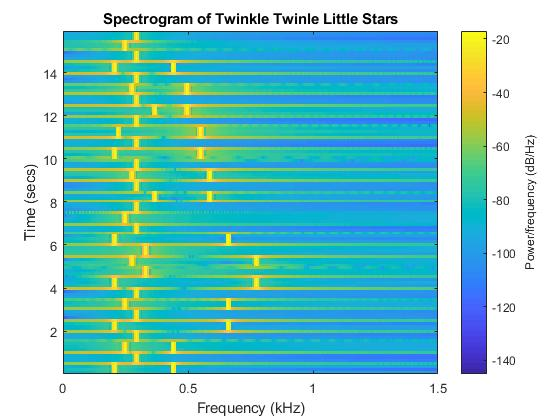
\includegraphics[scale=0.3]{task4b.jpg}
        \end{center}
        \begin{multicols}{2}
            \begin{center}
                C\\
                \columnbreak
                MATLAB
            \end{center}
        \end{multicols}
        Comparing the C-program result with the MATLAB result using relative error as the distance measure yields,
        \begin{center}
            \boxed{RelativeError = ||x-y|| = \frac{|measured-actual|}{measured}\times 100=21.86 \%}
        \end{center}
    \subsection{Task 8.} Implement the IIR filter in a C program. Write the result to a WAV file and read into MATLAB. Compare the C with the MATLAB implementation of the filtered song, \textit{Twinkle Twinkle Little Star}.
    \begin{center}
            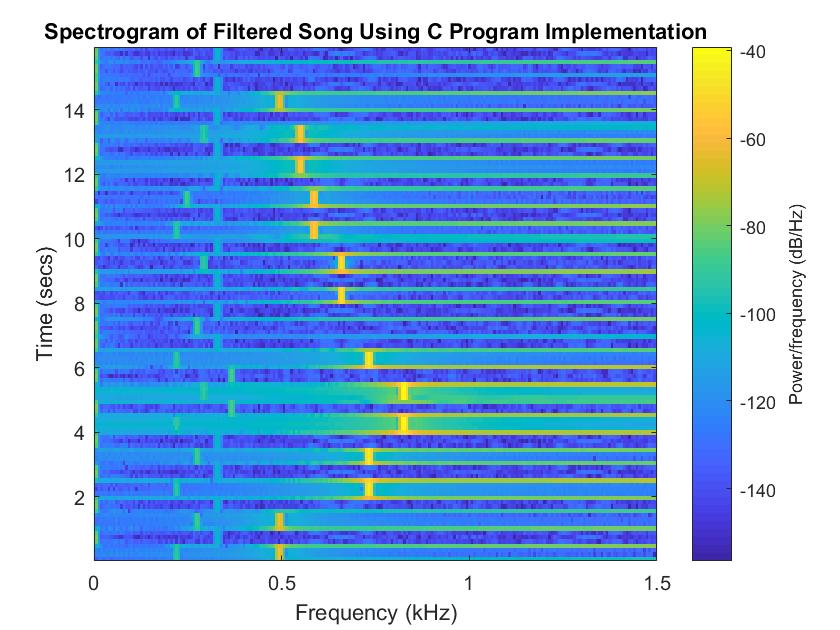
\includegraphics[scale=0.2]{task8a.jpg}
            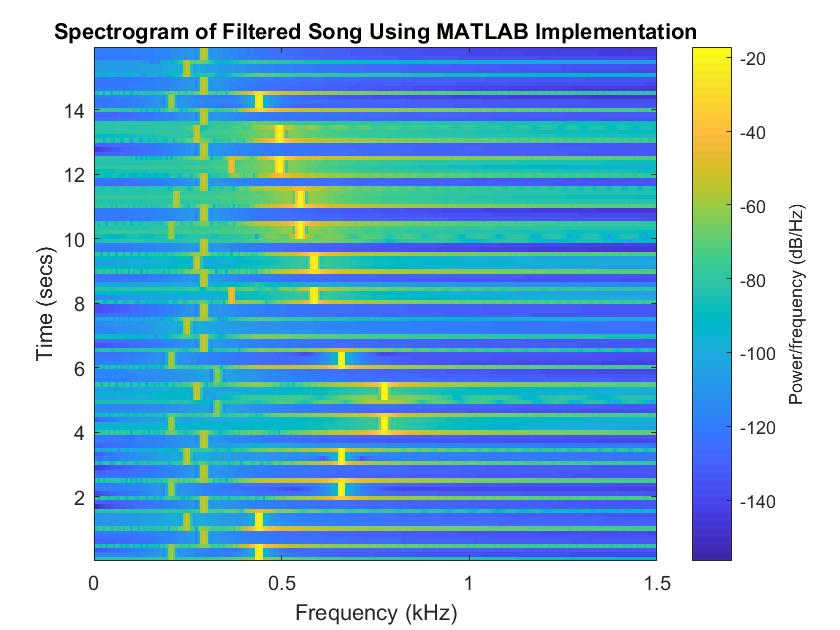
\includegraphics[scale=0.2]{task8b.jpg}
        \end{center}
        \begin{multicols}{2}
            \begin{center}
                C\\
                \columnbreak
                MATLAB
            \end{center}
        \end{multicols}
        \vspace{2mm}
        The C program implementation of the IIR is shown below.
        \begin{center}
            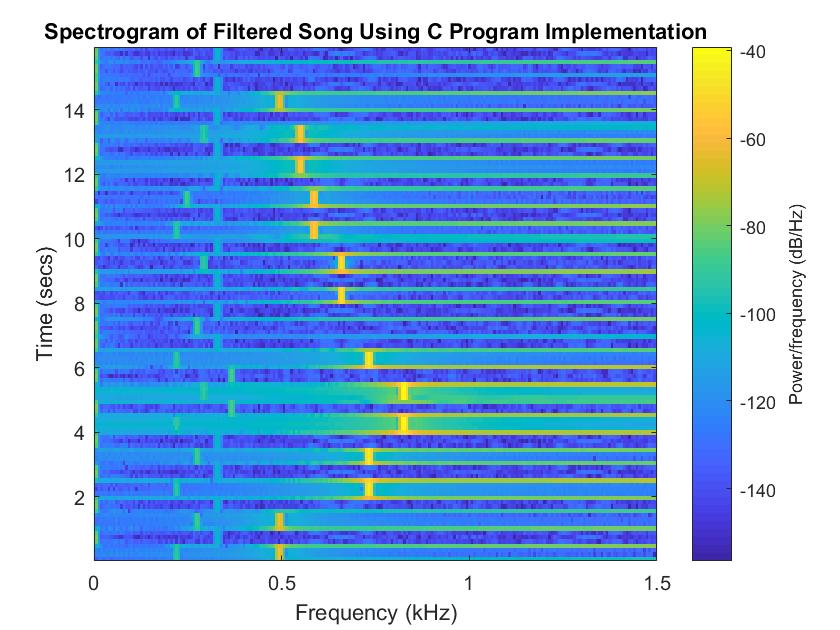
\includegraphics[scale=0.38]{task8a.jpg}
        \end{center}
        We can observe that the C implementation has reduced the power of all frequencies very slightly. The spectrogram confirms that the low frequencies have been filtered, as we can see the frequencies below 500Hz has become more blue--attenuated. Comparing the two, we can say that the C implementation has done a better job filtering out the low frequency components.
\newpage
\section{Code Appendix}
    \subsection{MATLAB Code:}
        \lstinputlisting[frame=single]{code-files/lab1.m}
        \vspace{5mm}
        \subsubsection{IIR-Filter Function}
        \lstinputlisting[frame=single]{code-files/IIR_filter_h.m} 
        %\begin{adjustbox}{max width=\textwidth}
        %    \lstinputlisting[frame=single]{code-files/lab1.m}
        %\end{adjustbox}
    \newpage
    \subsection{C Code:}
        \lstinputlisting[frame=single]{code-files/Lab1.c}
    \newpage
    \subsection{\LaTeX Code:}
        \lstinputlisting[frame=single]{main.tex}
\end{document}
